\section{Problem Setting}

Distributed system is hard to debug since some error can only be reproduced in some specific interleaving of sending and receiving massages between nodes. We try to synthesize a specialized scheduler to bias the scheduling to make the given blackbox model more likely to violate given specification. Then, this biased scheduler can be applied into real implementation to do more efficient testing.

In order to formalize 1) the non-deterministic choice of interleaving messages 2) the effectful essence of these messages, I define the state of whole system as a pair $(\alpha, s)$, where trace $\alpha$ is a sequence of \emph{received} messages and multi-set (we allow duplicate messages) $s$ contains all sent by not received messages. The transition between two states are
\begin{align*}
    (\alpha, s \uplus \{msg\}) \xrightarrow{(msg, s')} (\alpha \listconcat msg, s \cup s')
\end{align*}\noindent
which means that ``with a trace $\alpha$ and a multi-set of pending messages $s \uplus \{msg\}$, if scheduler makes message $msg$ to be received, the distributed system will send a multi-set of new messages $s'$, and reach a new state $(\alpha \listconcat msg, s \cup s')$''. We also can represent the execution above as a \emph{history}:
\begin{align*}
   (\Code{init}, s_0);(msg_1, s_1);(msg_2, s_2);...;(msg_n, s_n)
\end{align*}\noindent
where $\Code{init}$ is an initialization message that don't need to be send previously, and this history needs to satisfy well-formed relation that $msg_i$ is indeed a pending message at current stage. Note that, the semantics can be defined as an global automata.

\begin{figure}[h!]
    % https://tikzcd.yichuanshen.de/#N4Igdg9gJgpgziAXAbVABwnAlgFyxMJZARgBpiBdUkANwEMAbAVxiRAB13gYaB9YzgF8Qg0uky58hFACZSABiq1GLNp258ZQkWJAZseAkQDM5JfWatEHdjAC2aHAE84MHDvEGpReQvMqrGw1+UgACHl4tdmFBJRgoAHN4IlAAMwAnCDskXxAcCCQ5ZUs2AAoIslDOe0cXNwBKEGo4AAssVPdEXIY6ACMYBgAFCUNpEHSsBJb3UTTM7K7qfKQyYtVrcr5K9QiowUbqHv6hke9rLDBsWCaQfrAoJABaY3lZkAysnKWCxZAGCAgaB8pFSjFcSiOA2GXiM1gmU3c1As6xAmxCVS4FSEjTeHwWq2WiFMa0CaLkGOClV22JukJOMLG8OmHne8y+eR+xORpIqYR2WzC1OiON0eKQxMJxP+gKIMgA7L5QQxwYc+lDTrDxpNmUiAmVeRSscKANyhMl8zGaGm4tmIAk-VbSoEoYgADkVYJgELV9MkmqZiJJ+s0FuCexFc0+du+hV1JQ2uwtNWcrhwEdZUft7LuD0Qz1y3ODkVDRv2tJ90L9YwuV1YsUEQA
\begin{tikzcd}
{\{ev_1, ev_2\}} \arrow["{(ev_1, \{ev_1\}); (ev_2, \{ev_2\})}"', loop, distance=2em, in=215, out=145] &                                                                                                                                                                                                                & \{ev_2\} \arrow[ll, "{(ev_2, \{ev_1, ev_2\})}"'] \arrow["{(ev_2, \{ev_2\})}"', loop, distance=2em, in=125, out=55] \arrow[rd, "{(ev_2, \emptyset)}"] \arrow[ld, "{(ev_2, \{ev_1\})}" description, bend right] &           \\
                                                                                                      & \{ev_1\} \arrow[rr, "{(ev_1, \emptyset)}"'] \arrow[ru, "{(ev_1, \{ev_2\})}" description, bend right] \arrow["{(ev_1, \{ev_1\})}"', loop, distance=2em, in=305, out=235] \arrow[lu, "{(ev_1, \{ev_1, ev_2\})}"] &                                                                                                                                                                                                               & \emptyset
\end{tikzcd}
    \caption{An example of default declarative scheduler that represented as an automata.}
    \label{fig:scheduler-as-fa}
\end{figure}

\begin{example} Consider the scheduler automata shown in \autoref{fig:scheduler-as-fa}, whose states are sets of pending messages; we assume there are at most two pending messages to make the automata be finite. Traversing in this automata will lead well-formed histories. In this example, every state is both initial and final state (we can also have an explicit \Code{init} transition points to some states).
\end{example}

\begin{figure}
% https://tikzcd.yichuanshen.de/#N4Igdg9gJgpgziAXAbVABwnAlgFyxMJZABgBoBGAXVJADcBDAGwFcYkQAdD4GWgfXKlefAExcAviHGl0mXPkIpBxanSat2XHDAAeOAMYRGEAE7AARixjiLjevoDW5iDsnTZ2PASKCRqhlaaHNp6hsZmlqw2lvZOLm4yIBieCkQipH40ARqInNzC5BJSicny3ijpKlnqbLlcPPxiHAkeZYrIAMwU-jVBIQZGprZRtrHOrsWtXu0ALN3VgXUcMAC2aDgAnnAwOFKqMFAA5vBEoABmJhArSGQgOBBIgmqLICYw+rRcANwFIDTmMDAUBuNDsAMYAAU5NN2FgwNhYJMQBcriC7g9EOlnjlXu9PhwvgACYQiP4gMEwSHQ1K5OEItj-QHAxDEdzIy7XTE0e5ILrY2p5BoCIqg+jgqEpcqvLCHAAWuzZKM5Tx5LMZQKQAFoOrdsgL6gUReSxZSJW12CYZfKkUrHtyMXN+UFVustjsbRzefakABWBY4t4fb6-UXi6lSulYRHq5msxK2xCO1V+p25QP4n6NMkUqmSxQgSPRkAAjUsxWexAp1UANn9+uWa022wV8YrWNVtxLzJ1daCQqaLXZqMr3sTMa1PdTgpJRpzZphaatLfOFarGL5Xd5ut6SyFhWaHuHa7Rer7BVIxMas5NufNi7lCso4iAA
\begin{tikzcd}
                                                                                           & \textcolor{blue}{blackbox} \arrow[ld, "\{ev_1\}"', bend right] \arrow[r, "\emptyset"] & \{ev_2\} \arrow[rd, "recv\;ev_2" description] &                                                                                                                                                          &           \\
{\{ev_1,ev_2\}} \arrow[ru, "recv\;ev_1" description] \arrow[rd, "recv\; ev_2" description] &                                                                                       &                                               & \textcolor{blue}{blackbox} \arrow[r, "\emptyset"] \arrow[lu, "\{ev_2\}"', bend right] \arrow[ld, "\{ev_1\}", bend left] \arrow[lll, "{\{ev_1, ev_2\}}"'] & \emptyset \\
                                                                                           & \textcolor{blue}{blackbox} \arrow[r, "\{ev_1\}"'] \arrow[lu, "\{ev_2\}", bend left]   & \{ev_1\} \arrow[ru, "recv\;ev_1" description] &                                                                                                                                                          &          
\end{tikzcd}    
\caption{An example of default operational scheduler that represented as an automata.}
    \label{fig:scheduler-as-ofa}
\end{figure}

In the runtime, a operational scheduler divide the scheduling and the execution of blackbox model as shown in \autoref{fig:scheduler-as-ofa}. A action $(ev, \{ev_i\})$ is divided into two phases, the scheduler choose messages to receive (e.g., $ev$), and the blackbox model chooses what messages to send after receive (e.g., $\{ev_i\}$). If the choice of blackbox model violates the expectation of the scheduler, the execution will just stop (it can cause by violation of specification, or violation of axioms, it is also a monitor). The special initialization action $(\Code{init}, ev)$ is fully controlled by the scheduler (i.e., when scheduler chooses \Code{init}, the messages $\{ev\}$ is sent by scheduler itself).

\paragraph{Problem Statement} For given specification $\phi$ and system model $P$, a set of execution sampling of $P$ as $S$, we try to specifies the default scheduler automata $A$ into $A'$ with an axiom $\psi$ for blackbox model, where $A' \subseteq A$, $A'$ is consistent with $S$, and every trace accepted by $A'$ will violate $\phi$.

\paragraph{Guarantee: Well-formed Scheduler} We guarantee all automata-based scheduler will not schedule messages in impossible way -- receiving message without sending it.

\paragraph{Guarantee: Safety} We guarantee if an scheduler $A$ is biased into $A'$, $A' \subseteq A$. 

\paragraph{Guarantee: Axiom Correctness} If axiom $\psi$ for blackbox model is consistent with execution sampling $S'$.

\paragraph{Guarantee: Relatively Reliability} If axiom $\psi$ for blackbox model holds, all history scheduled by $A'$ is realizable and leads to bugs.

In practical, we can continue update new scheduler, sampling new traces, and use these traces to biased scheduler -- we should use experiment to show it.

\section{Motivating Example}

Consider a Read-Write example. Assume there are two users tries to write a boolean cell in the system that has no consistency guarantee. There are $4$ APIs:
{\footnotesize\begin{align*}
    &\Code{readReq: \{nodeId: int;\}}\\
    &\Code{writeReq: \{nodeId: int; va: bool\}}\\
    &\Code{readRsp: \{nodeId: int; va: bool\}}\\
    &\Code{writeRsp: \{nodeId: int; va: bool\}}
\end{align*}}\noindent
On possible implementation can be
\begin{minted}[xleftmargin=5pt, numbersep=4pt, linenos = true, fontsize = \footnotesize, escapeinside=??]{OCaml}
let cell = ref 0
let model = function
    | readReq {nodeId} -> send (readRsp {nodeId; va = !cell})
    | writeReq {nodeId; va} ->
        cell := va; send (writeRsp {nodeId; va = !cell})
\end{minted}
We treat to prove the specification that ``for each node (indicates a user), the received read response has the same vaue with the last write response.''. Then the negation of this specification is
{\footnotesize\begin{align*}
    &\exists \Code{i{:}int}.\exists \Code{b{:}bool}. 
    \\&\Code{writeRsp(nodeId = i \land va = b);(\bullet \setminus writeRsp(nodeId = i))^*;readRsp(nodeId = i \land va \not= b)}
\end{align*}}\noindent
Then an execution violates this specification can be
{\footnotesize\begin{align*}
    &\Code{(init, \{\textcolor{blue}{writeReq(0,true)}\})};
    \\&\Code{(init, \{\textcolor{DeepGreen}{writeReq(1, false)}\})};
    \\&\Code{(\textcolor{blue}{writeReq(0,true)}, \{\textcolor{red}{writeRsp(0,true)}\})};
    \\&\Code{(\textcolor{red}{writeRsp(0,true)}, \emptyset)};
    \\&\Code{(init, \{\textcolor{codepurple}{readReq(0)}\})};
    \\&\Code{(\textcolor{DeepGreen}{writeReq(1, false)}, \{writeRsp(1, false)\})};
    \\&\Code{(\textcolor{codepurple}{readReq(0)}, \{\textcolor{codeblue}{readRsp(0, false)}\})};
    \\&\Code{\textcolor{codeblue}{readRsp(0, false)}, \emptyset)};
\end{align*}}\noindent
where the sending and receiving of the same message is using the same color.

Then, by symbolization, we have $2+4+4+4 = 14$ symbolic events.
{\footnotesize\begin{align*}
    &0:\Code{readReq(nodeId = i), 1:readReq(nodeId \not= i)\}}\\
    &2:\Code{writeReq(nodeId = i \land va = b), 3:writeReq(nodeId = i \land va \not= b), 4:writeReq(nodeId \not= i \land va = b) ...}\\
    &\Code{6:readRsp(nodeId = i \land va = b), 7:readRsp(nodeId = i \land va \not= b), 8:readRsp(nodeId \not= i \land va = b) ...}\\
    &\Code{10:writeRsp(nodeId = i \land va = b), 11:writeRsp(nodeId = i \land va \not= b), 12:writeRsp(nodeId \not= i \land va = b) ...}
\end{align*}}\noindent

Assume that we allow at most two pending messages, the default scheduler show as below (some edges are omitted).

\begin{center}
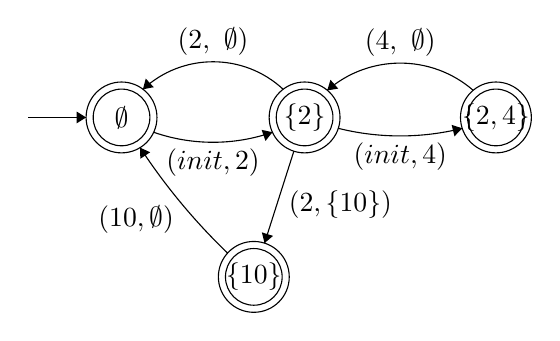
\begin{tikzpicture}[scale=0.15]
\tikzstyle{every node}+=[inner sep=0pt]
\draw [black] (15.5,-18.2) circle (3);
\draw (15.5,-18.2) node {$\emptyset$};
\draw [black] (15.5,-18.2) circle (2.4);
\draw [black] (31,-18.2) circle (3);
\draw (31,-18.2) node {$\{2\}$};
\draw [black] (31,-18.2) circle (2.4);
\draw [black] (47.2,-18.2) circle (3);
\draw (47.2,-18.2) node {$\{2,4\}$};
\draw [black] (47.2,-18.2) circle (2.4);
\draw [black] (26.7,-31.7) circle (3);
\draw (26.7,-31.7) node {$\{10\}$};
\draw [black] (26.7,-31.7) circle (2.4);
\draw [black] (28.28,-19.455) arc (-70.83829:-109.16171:15.325);
\fill [black] (28.28,-19.45) -- (27.36,-19.25) -- (27.69,-20.19);
\draw (23.25,-20.8) node [below] {$(init,2)$};
\draw [black] (44.348,-19.123) arc (-76.01975:-103.98025:21.723);
\fill [black] (44.35,-19.12) -- (43.45,-18.83) -- (43.69,-19.8);
\draw (39.1,-20.27) node [below] {$(init,4)$};
\draw [black] (17.306,-15.823) arc (132.92756:47.07244:8.728);
\fill [black] (17.31,-15.82) -- (18.23,-15.64) -- (17.55,-14.91);
\draw (23.25,-12.99) node [above] {$(2,\mbox{ }\emptyset)$};
\draw [black] (32.917,-15.909) arc (130.96442:49.03558:9.431);
\fill [black] (32.92,-15.91) -- (33.85,-15.76) -- (33.19,-15.01);
\draw (39.1,-13.1) node [above] {$(4,\mbox{ }\emptyset)$};
\draw [black] (30.09,-21.06) -- (27.61,-28.84);
\fill [black] (27.61,-28.84) -- (28.33,-28.23) -- (27.38,-27.93);
\draw (29.62,-25.61) node [right] {$(2,\{10\})$};
\draw [black] (7.6,-18.2) -- (12.5,-18.2);
\fill [black] (12.5,-18.2) -- (11.7,-17.7) -- (11.7,-18.7);
\draw [black] (24.479,-29.684) arc (-133.87969:-146.7601:51.717);
\fill [black] (17.07,-20.76) -- (17.09,-21.7) -- (17.93,-21.15);
\draw (19.97,-26.86) node [left] {$(10,\emptyset)$};
\end{tikzpicture}
\end{center}

As we know, some edges are impossible (e.g., $(2, \emptyset)$ indicates handler of $\Code{writeReq(nodeId = i \land va = b)}$ will not send any message); some edges cannot reach to erroneous state, for example, 
\begin{align*}
    (init,\{2\});(2,\{10\});(10,\{\emptyset\})
\end{align*}
The specified scheduler should rule out these histories.

\section{Axioms}

\begin{align*}
    \forall x. \{A\}\;ev\;\{S\}
\end{align*}
When receiving an event $v$ will sends a set of messages $s$, it \emph{must} has prefix trace accepted by $A$ -- an underapproximated-style specification.
\begin{align*}
    \forall \Code{id\;v}. \{\bullet^*;writeRsp(\_, v);(\bullet \setminus writeRsp(\_, \_))^*\}\;\Code{readReq(id)}\;\{\{readRsp(id, v)\}\}
\end{align*}
The $S$ can be extracted from the samples, however, the $A$ need to be reasonable synthesized (instead of using set of sampled traces).